\documentclass[12pt,a4paper]{article}
\usepackage[utf8]{inputenc}
\usepackage[spanish]{babel}
\usepackage{amsmath}
\usepackage{amsfonts}
\usepackage{amssymb}
\usepackage{makeidx}
\usepackage{graphicx}
\usepackage{multicol}
\usepackage{changepage}
\usepackage{float}
\usepackage{cite}
\usepackage{url}
\usepackage[left=2cm,right=2cm,top=2cm,bottom=2cm]{geometry}

\begin{document}
%encabezado 
\pagestyle{plain}{
\pagestyle{empty}
\changepage{3cm}{1cm}{-0.5cm}{-0.5cm}{}{-2cm}{}{}{}
\noindent
{
\small
\begin{tabular}{p{0.75\textwidth} p{0.25\textwidth} }

\includegraphics[scale=0.3]{logoUniversidad.png}&
\includegraphics[scale=0.5]{images.jpg} 
\end{tabular}
}
%datos de la caratula
\begin{center}
\par\vspace{2cm} %Rspacoo dejado antes del encabezado
{
\Huge\textbf{
Universidad de Guayaquil \\*[0.40cm] Facultad de Ciencias Matem\'aticas y F\'isicas}
}
\par\vspace{2cm}
{
\Large\textbf{Integrantes:}
\par\vspace{0.2cm}
\Large\textbf{Chiriguaya Alvaro}\\
\Large\textbf{Mite Lady} \\
\Large\textbf{Zambrano Alisson}\\
\par\vspace{0.5cm}
\Large\textbf{Proyecto basado en la norma ISO 9001:20152}
\par\vspace{1cm}
\Large\textbf{Ingenier\'ia de Software}
\par\vspace{1cm}
\Large\textbf{Materia: Procesos de Software}
\par\vspace{1cm}
\Large\textbf{Docente: Ing. Miguel \'Angel Botto Tobar }
}
\par\vspace{2cm}
\large\textbf{ 4/03/2020}
\par\vspace{0.5cm}
\large\textbf{2019-2020} 
\par\vspace{3cm} 

\end{center}
\clearpage
}

\tableofcontents
\par\vspace{12cm}

\section{Normas ISO 9001}\textbf{}
La Norma ISO 9001:2015 es la base del Sistema de Gestión de la Calidad - SGC. Es una norma internacional que se centra en todos los elementos de la gestión de la calidad con los que una empresa debe contar para tener un sistema efectivo que le permita administrar y mejorar la calidad de sus productos o servicios. 
Los clientes se inclinan por los proveedores que cuentan con esta acreditación porque de este modo se aseguran de que la empresa seleccionada disponga de un buen SGC.

\section{Caso de estudio}\textbf{}
El TPV o POS (Point of Sale) es la evolución del siglo XXI de la clásica caja registradora. En el mundo de la hostelería y venta al por menor de pequeños comercios los TPV son utilizados para registrar ventas, beneficios, pedidos, inventarios, historial de clientes, etc. En resumen, un TPV otorga control sobre las operaciones de negocio.\\
Un TPV básico consiste en una computadora, un cajón de dinero, una impresora de tiques, un monitor y dispositivos de lectura como lector de códigos de barras, teclados, etc. Los TPV registran las transacciones y permiten generar detallados informes, permitiendo tomar mejores decisiones comerciales. El TPV correcto permitirá mejorar la productividad y redundará en mejores ganancias.\\
Un TPV puede revolucionar el funcionamiento de un comercio. Desde incrementar la productividad de los empleados hasta conocer si las inversiones obtienen beneficios.\\\\

\section{Sistema de gestión de calidad}\textbf{}
\subsection{Objeto y campo de aplicación}
Elaboración de un programa que sea ideal para la venta de comidas rápidas (pizzerias, hamburgueserias, bocadillerías, etc.). En donde se permita lo siguiente:
\begin{itemize}
\item Registra los datos del cliente.
\item Realizar pedidos a domicilio.
\item Gestiona los consumos de los clientes en el propio local.
\item Opción a que el cliente pueda el pedido telefónicamente y en lugar de servirle al domicilio viene a recogerlo al local.
\item Atención de pedidos en las mesas del local, de forma directa.
\item Permitir imprimir los listados para gestionar los temas del negocio. Entre otros: presupuestos, facturas realizadas, gastos, beneficios, listados de impuestos, etc.
\end{itemize}
\begin{center}

\includegraphics[width=0.6\textwidth]{primeraimagen.jpg}  
\end{center}

\section{Referencias normativas}\textbf{}
ISO 9001: 2015, Sistemas de gestión de calidad. Fundamentos y vocabulario.

\section{Términos y definiciones}\textbf{}
Para los fines de este documento, aplican los términos y definiciones incluidos en la norma ISO 9001:2015 y los de la empresa especialista en la creación y venta de software “TPV Gratuito 123”.
\begin{center}
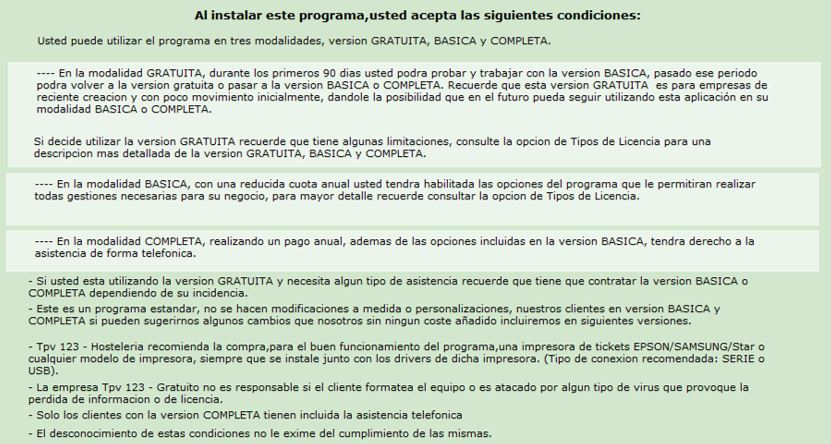
\includegraphics[width=0.9\textwidth]{segundaimagen.jpeg}   
\end{center}

\section{Contexto de la organización}\textbf{}
El objetivo de la empresa es ayudar a los clientes a ahorrar tiempo y dinero en las gestiones diarias de su negocio, proporcionando sencillez y fiabilidad en sus gestiones, permitiéndoles concentrarse en la lógica de su negocio.
Se esfuerzan en introducir nuevas e interesantes características en nuestros productos.
Escuchan las peticiones de nuestros clientes para adaptar nuestras soluciones y satisfacer el mercado.
 Los TPV de la empresa son ampliamente utilizados por cientos de empresas en el mundo.
 Las opciones más necesarias y básicas son gratuitas.
 Dan cobertura a prácticamente todo tipo de negocios.
 Soporte técnico especializado en atender tus dudas e incidencias.
 
\subsection{Determinación del alcance}
El programa es ideal si el negocio de restaurante está orientado a Comida Rápida o también con el conocido término de FastFood. Es decir que podrá ser implementado en restaurantes como:
\begin{itemize}
\item Pizzerías
\item Hamburgueserías
\item Bocadillerías
\item Taquerías\\\\
\end{itemize}

\subsection{Procesos}
El programa cuenta con los siguientes procesos:
Pedidos a domicilio.
\begin{itemize}
\item Consumo en local.
\item Pedido telefónico y recogida en local.
\item Servicio en mesa.
\item Caja.
\item Listados.\\\\
\end{itemize}

\section{Liderazgo}\textbf{}
\subsection{Liderazgo y compromiso}
\textbf {Generalidades del sistema}\\\\
El menú principal del programa nos indica las opciones principales que tiene la aplicación y la intención de modular hace todo lo posible para que su utilización sea la más fácil y ágil, este contiene lo siguiente:
\begin{itemize}
\item Proveedores
\item Familias
\item Productos
\item Empleados
\item Clientes
\item Caja
\item Stock
\item Configuración
\item Listados
\item Acerca de
\item Nivel de acceso\\\\
\end{itemize}

\textbf {Enfoque al cliente}\\\\
Gracias al modularidad que ofrece nuestro programa en el apartado de clientes se puede observar que cuenta con los campos necesarios para el registro exitoso de los mismos, los campos son los siguientes: 
\begin{itemize}
\item Teléfono Móvil 
\item Nombre del cliente
\item Apellidos del cliente
\item Dirección del cliente 
\item Población del cliente
\item D.N.I del cliente 
\item Provincia del cliente 
\item C.P.
\item E-Mail
\item Atendido por 
\item Ultima visita 
\end{itemize}

Además, este apartado permite mostrar la lista de clientes, la cual se muestra de una forma ordenada por medio de una tabla que cuenta con 4 celdas las cuales son:
\begin{itemize}
\item Teléfono 
\item Móvil
\item Nombre del cliente
\item Fecha Alta 
\end{itemize}

Esta lista se puede ordenar por nombre, por fecha de Alta y por número de teléfono.
Este aparatado cuenta con las opciones de modificar, Añadir un nuevo cliente, Buscar cliente, eliminar cliente y salir.

\subsection{Políticas}
\textbf{Comunicación de la política de calidad}\\\\
La información del programa está disponible en la página de la empresa y cuenta con los manuales necesarios para la utilización de este.
El programa también cuenta con dos versiones de pago, las cuales dan acceso a llamadas telefónicas para servicio al cliente mientras que la versión básica, es decir la gratuita cuenta con servicio al cliente por vía mensajería; manteniendo así contacto la empresa desarrolladora del producto y el cliente.

\subsection{Roles y responsabilidades}
\textbf {Proveedores:} Una de las condiciones para que un software funcione es la introducción de dato, por ello uno de los primeros pasos a seguir es dar de alta los proveedores con los que se pretende trabajar.\\\\
\textbf {Familias:} Con este módulo del programa se crearán las familias del programa, con familia se refiere a la agrupación de productos homogéneos para la venta. En este apartado de familias se detallará en que consiste cada opción que maneja.\\\\
\textbf {Productos:} Aunque el programa tiene unos datos de prueba, en su versión prueba no dejan de ser datos que en la mayoría de ellos se tendrá que cambiar el nombre y el precio, así como sus imágenes o colores a utilizar en el programa.\\\\
\textbf {Empleados:} Daremos de alta a todos los empleados del negocio pudiendo darle a cada uno de ellos los permisos necesarios a cada usuario.\\\\
\textbf {Clientes:} Si la empresa necesita o cree conveniente dar de alta a los clientes puede hacerlos desde esta modulo del programa, que también se accederá a él desde el módulo de caja para los pedidos telefónicos o para entregar una factura del consumo que hayamos hecho.\\\\
\textbf {Caja:} Este será el aparatado del programa donde más tiempo se utilizará el programa. Este módulo se encarga de realizar las ventas de nuestros productos. En cada ventana de este módulo se encontrarán unos botones de ayuda que se recomienda utilizar al menos en la fase de implementación.\\\\
\textbf {Stock:} Desde este apartado se manejará todo lo relacionado por con el Stock y Almacén del negocio, así como inventarios y movimientos de productos algunos listados.\\\\
\textbf {Configuración:} Esta herramienta será utilizada por el propietario del negocio o encargado para parametrizar cada apartado del programa permisos, idiomas, colores del programa, claves de acceso, copias de seguridad, creación de salones, alta de impresoras, tipo de impuestos, creación de barras, horarios de cocina, etc.\\\\
\textbf {Listados:} La relación de listados y gráficos de ventas del negocio ayudarán a tomar decisiones para la optimización del negocio.\\\\
\textbf {Acerca de:} Desde esta opción del programa veremos algunos datos de la empresa desarrolladora del software, así como la situación de la licencia de uso del programa, es importante no dejar de leer las condiciones y utilización del programa, es indispensable recordar que este es un software comercial y que su utilización es bajo licencia de la empresa SOLVERMEDIA que tiene registrado los derechos en marca y patentes tanto en contenido y diseño.\\\\
\textbf {Asistencia/Soporte:} Sirve para poder enviar una consulta de forma rápida desde el programa.\\\\
\textbf {Tipo de licencia:} Desde aquí se puede ver que es lo que incluye cada uno de los tipos de registro para poder ver cuál es el que más se adapta a la forma de trabajo en el caso de que se quiera ver la compra.\\\\
\textbf {Activar licencia:} Realiza el registro de la licencia.\\\\
\textbf {Condiciones de uso:} Aquí se visualiza cuales son las condiciones de uso del programa.\\\\
\textbf {Conectar en red:} Aquí se puede ver el manual de conexión.
\par\vspace{0.5cm}

\section{Planificación}\textbf{}
Al realizar el SGC, la empresa consideró varios puntos importantes, como lo son el alcance, los procesos y los requerimientos referidos, para así determinar los riesgos y oportunidades que se van a abordar con la finalidad de:
\begin{itemize}
\item Asegurar que se cumplan los resultados
\item Aumentar los efectos deseables
\item Prevenir o reducir los efectos no deseados
\item Lograr mejoras
\end{itemize}
Las acciones tomadas para abordar los riesgos y oportunidades son proporcionales al impacto potencial en la conformidad del producto que brinda la empresa.

\section{Apoyo}\textbf{}
El programa cuenta con un apartado de Asistencia y Sugerencia, en donde aparecerá una interfaz en la que se podrá realizar dos tipos de consulta:
\begin{itemize}
\item Pregunta o Consulta
\item Aviso de avería
\end{itemize}
Si el usuario selecciona cualquiera de estas dos opciones aparecerá una caja de texto en la cual se podrá formular la consulta y para culminar la consulta se deberá ingresar los datos, de esta forma la empresa brindará una respuesta.\\\\
En caso de no recibir una respuesta también se podrá comunicar con el departamento de Asistencia y Consultas de la empresa al número telefónico:   +34.91.142.62.02 (Madrid – España).

\section{Operación}\textbf{}
El programa cuenta con tres tipos de Licencia:

\begin{itemize}
\item Licencia Gratuita (0,00 euros)
\item Licencia Básica (49,00 euros)
\item Licencia Completa (110,00 euros)\\
\end{itemize}

Dentro de la Licencia Gratuita encontramos las siguientes características:

\begin{itemize}
\item \textbf {Asistencia por Email:} No Incluido
\item \textbf {Asistencia Telefónica:} No Incluido
\item \textbf {Proveedores:} Máximo 20
\item \textbf {Productos:} Máximo 250
\item \textbf {Alta de Familias:} Sin límite
\item \textbf {Alta de Menús:} Sin límite
\item \textbf {Empleados:} Máximo 4
\item \textbf {Comisiones para Empleados:} Incluido
\item \textbf {Clientes:} No Incluido
\item \textbf {Caja:} Máximo 20 Ventas / día
\item \textbf {Envío de pedidos a Cocina:} Incluido
\item \textbf {Juntar Cuentas:} No Incluido
\item \textbf {Cobro Parcial:} No Incluido
\item \textbf {Observaciones de Pedido:} No Incluido
\item \textbf {Promociones:} Incluido
\item \textbf {Conteo y Cierre de Caja:} Incluido
\item \textbf {Modificación o Reimpresión de Ticket de Venta:} Incluido
\item \textbf {Activar precios para este terminal de venta:} No Incluido
\item \textbf {Gastos del día:} No Incluido
\item \textbf {Retiradas de caja:} No Incluido
\item \textbf {Mantenimiento y Formas de Pago:} Incluido
\item \textbf {Imprimir PreTickets:} Incluido
\item \textbf {Reemprimir Ticket:} No Incluido
\item \textbf {Emitir Facturas:} No Incluido
\item \textbf {Listados:} No Incluido
\item \textbf {Venta con código de barras:} No Incluido
\item \textbf {Stock:} No Incluido
\item \textbf {Selección de tipo de IVA (Incluido/No Incluido):} Incluido
\item \textbf {Hacer copia de Seguridad:} Incluido
\item \textbf {Alta de Impresoras:} Incluido
\item \textbf {Cambiar de Idioma:} Incluido
\item \textbf {Configuración de monedas, decimales, impuestos de su país:} Incluido
\item \textbf {Asistencia/Soporte:} No Incluido
\item \textbf {Creación de salones:} Incluido
\item \textbf {Creación de Barras:} Incluido
\item \textbf {Permisos de Usuario:} No Incluido
\item \textbf {Enviar resumen de ventas por email:} No Incluido
\item \textbf {Eliminar datos de pruebas:} Incluido

\item \textbf {Aumento de impuestos:} No Incluido
\item \textbf {Configurar Horario Atención al Público:} No Incluido
\item \textbf {Configurar Horarios de Cocina:} No Incluido
\item \textbf {Diseño de Ticket:} Incluido
\item \textbf {Niveles de Acceso:} No Incluido
\item \textbf {Configuración apertura cajetín de monedas:} Incluido
\item \textbf {Listados en Formato Ticket:} Incluido
\item \textbf {Listados Generales:} Incluido
\item \textbf {Listados Estadísticas/Gráficos:} No Incluido
\item \textbf {Listado Ventas – Formato Folio:} No Incluido
\item \textbf {Cierre de año:} Incluido
\item \textbf {Aumento de Impuestos / Precios:} No Incluido\\\\\\\\\\
\end{itemize}

Dentro de la Licencia Básica encontramos las siguientes características:

\begin{itemize}
\item \textbf {Asistencia por Email:} Si Incluido
\item \textbf {Asistencia Telefónica:} No Incluido
\item \textbf {Proveedores:} Sin límite
\item \textbf {Productos:} Sin límite
\item \textbf {Alta de Familias:} Sin límite
\item \textbf {Alta de Menús:} Sin límite
\item \textbf {Empleados:} Sin límite
\item \textbf {Comisiones para Empleados:} Incluido
\item \textbf {Clientes:} Incluido
\item \textbf {Caja:} Sin límite
\item \textbf {Envío de pedidos a Cocina:} Incluido
\item \textbf {Juntar Cuentas:} Incluido
\item \textbf {Cobro Parcial:} Incluido
\item \textbf {Observaciones de Pedido:} Incluido
\item \textbf {Promociones:} Incluido
\item \textbf {Conteo y Cierre de Caja:} Incluido
\item \textbf {Modificación o Reimpresión de Ticket de Venta:} Incluido
\item \textbf {Activar precios para este terminal de venta:} Incluido
\item \textbf {Gastos del día:} Incluido
\item \textbf {Retiradas de caja:} Incluido
\item \textbf {Mantenimiento y Formas de Pago:} Incluido
\item \textbf {Imprimir PreTickets:} Incluido
\item \textbf {Reemprimir Ticket:} Incluido
\item \textbf {Emitir Facturas:} Incluido
\item \textbf {Listados:} Incluido
\item \textbf {Venta con código de barras:} Incluido
\item \textbf {Stock:} Incluido
\item \textbf {Selección de tipo de IVA (Incluido/No Incluido):} Incluido
\item \textbf {Hacer copia de Seguridad:} Incluido
\item \textbf {Alta de Impresoras:} Incluido
\item \textbf {Cambiar de Idioma:} Incluido
\item \textbf {Configuración de monedas, decimales, impuestos de su país:} Incluido
\item \textbf {Asistencia/Soporte:} Incluido
\item \textbf {Creación de salones:} Incluido
\item \textbf {Creación de Barras:} Incluido
\item \textbf {Permisos de Usuario:} Incluido
\item \textbf {Enviar resumen de ventas por email:} Incluido
\item \textbf {Eliminar datos de pruebas:} Incluido
\item \textbf {Aumento de impuestos:} Incluido
\item \textbf {Configurar Horario Atención al Público:} Incluido
\item \textbf {Configurar Horarios de Cocina:} Incluido
\item \textbf {Diseño de Ticket: }Incluido
\item \textbf {Niveles de Acceso:} Incluido
\item \textbf {Configuración apertura cajetín de monedas:} Incluido
\item \textbf {Listados en Formato Ticket:} Incluido
\item \textbf {Listados Generales:} Incluido
\item \textbf {Listados Estadísticas/Gráficos:} Incluido
\item \textbf {Listado Ventas – Formato Folio:} Incluido
\item \textbf {Cierre de año:} Incluido
\item \textbf {Aumento de Impuestos / Precios:} Incluido
\end{itemize}

Dentro de la Licencia Completa encontramos las siguientes características:

\begin{itemize}
\item \textbf {Asistencia por Email: }Si Incluido
\item \textbf {Asistencia Telefónica:} Si Incluido
\item \textbf {Proveedores:} Sin límite
\item \textbf {Productos:} Sin límite
\item \textbf {Alta de Familias:} Sin límite
\item \textbf {Alta de Menús:} Sin límite
\item \textbf {Empleados:} Sin límite
\item \textbf {Comisiones para Empleados:} Incluido
\item \textbf {Clientes:} Incluido
\item \textbf {Caja:} Sin límite
\item \textbf {Envío de pedidos a Cocina:} Incluido
\item \textbf {Juntar Cuentas:} Incluido
\item \textbf {Cobro Parcial:} Incluido
\item \textbf {Observaciones de Pedido:} Incluido
\item \textbf {Promociones:} Incluido
\item \textbf {Conteo y Cierre de Caja:} Incluido
\item \textbf {Modificación o Reimpresión de Ticket de Venta:} Incluido
\item \textbf {Activar precios para este terminal de venta:} Incluido
\item \textbf {Gastos del día:} Incluido
\item \textbf {Retiradas de caja:} Incluido
\item \textbf {Mantenimiento y Formas de Pago:} Incluido
\item \textbf {Imprimir PreTickets:} Incluido
\item \textbf {Reemprimir Ticket:} Incluido
\item \textbf {Emitir Facturas:} Incluido
\item \textbf {Listados:} Incluido
\item \textbf {Venta con código de barras:} Incluido
\item \textbf {Stock:} Incluido
\item \textbf {Selección de tipo de IVA (Incluido/No Incluido):} Incluido
\item \textbf {Hacer copia de Seguridad:} Incluido
\item \textbf {Alta de Impresoras: }Incluido
\item \textbf {Cambiar de Idioma: }Incluido
\item \textbf {Configuración de monedas, decimales, impuestos de su país:} Incluido
\item \textbf {Asistencia/Soporte:} Incluido
\item \textbf {Creación de salones:} Incluido
\item \textbf {Creación de Barras:} Incluido
\item \textbf {Permisos de Usuario:} Incluido
\item \textbf {Enviar resumen de ventas por email:} Incluido
\item \textbf {Eliminar datos de pruebas: }Incluido
\item \textbf {Aumento de impuestos:} Incluido
\item \textbf {Configurar Horario Atención al Público:} Incluido
\item \textbf {Configurar Horarios de Cocina: }Incluido
\item \textbf {Diseño de Ticket: }Incluido
\item \textbf {Niveles de Acceso:} Incluido
\item \textbf {Configuración apertura cajetín de monedas:} Incluido
\item \textbf {Listados en Formato Ticket:} Incluido
\item \textbf {Listados Generales: }Incluido
\item \textbf {Listados Estadísticas/Gráficos:} Incluido
\item \textbf {Listado Ventas – Formato Folio:} Incluido
\item \textbf {Cierre de año: }Incluido
\item \textbf {Aumento de Impuestos / Precios:} Incluido\\\\
\end{itemize}

\subsection{Diseño del producto}
\par\vspace{0.5cm}
\textbf {Inicio del Programa de FastFood}\\\\
\begin{center}
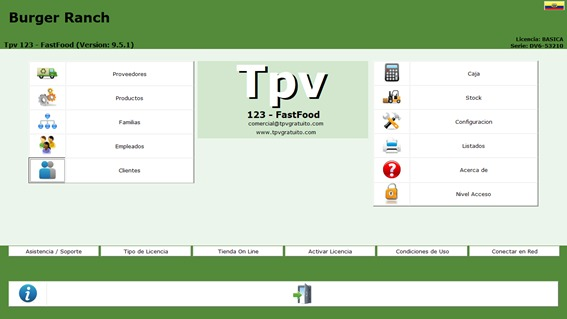
\includegraphics[scale=0.7]{1.jpg}
\end{center}
\par\vspace{6cm}
\textbf {Proveedores}\\\\
\begin{center}
 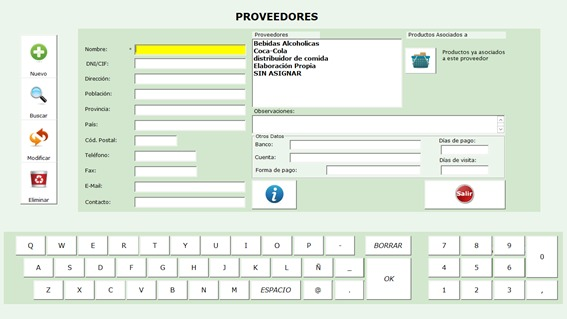
\includegraphics[scale=0.7]{2.jpg}
 \end{center} 
 \par\vspace{0.5cm}
\textbf {Familias}\\\\
\begin{center}
 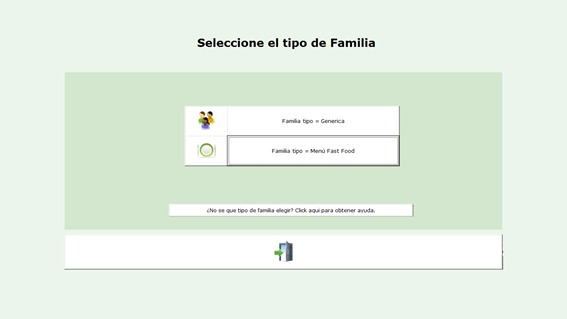
\includegraphics[scale=0.7]{3.jpg} 
 \end{center}
 \par\vspace{6cm}
\textbf {Productos}\\\\
\begin{center}
 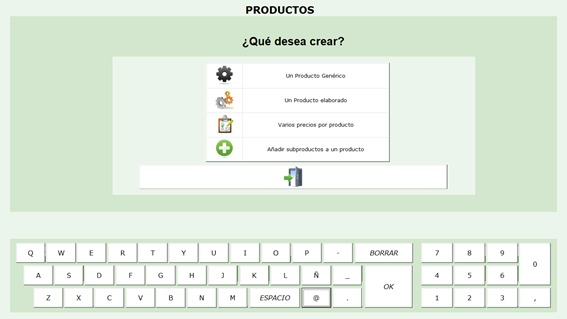
\includegraphics[scale=0.7]{4.jpg} 
 \end{center}
 \par\vspace{0.5cm}
\textbf {Empleados}\\\\
\begin{center}
 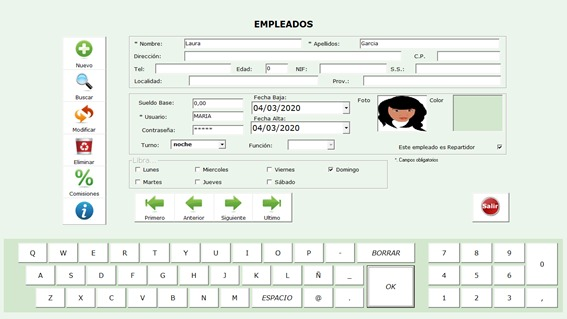
\includegraphics[scale=0.7]{5.jpg} 
 \end{center}
 \par\vspace{6cm}
\textbf {Clientes}\\\\
\begin{center}
 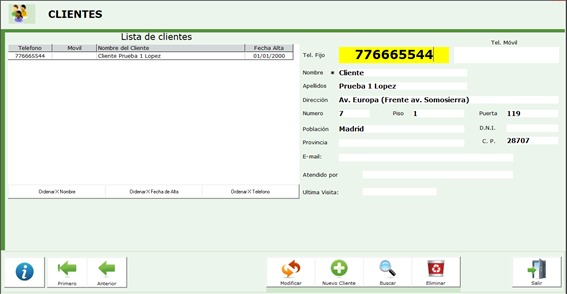
\includegraphics[scale=0.7]{6.jpg} 
 \end{center}
 \par\vspace{0.5cm}
\textbf {Caja}\\\\
\begin{center}
 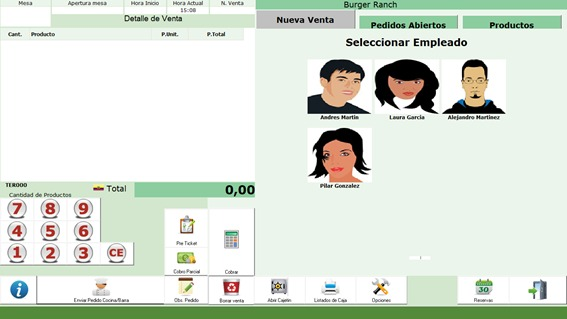
\includegraphics[scale=0.7]{7.jpg} 
 \end{center}
 \par\vspace{6cm}
\textbf {Stock, Pedidos y Movimientos de Productos}\\\\
\begin{center}
 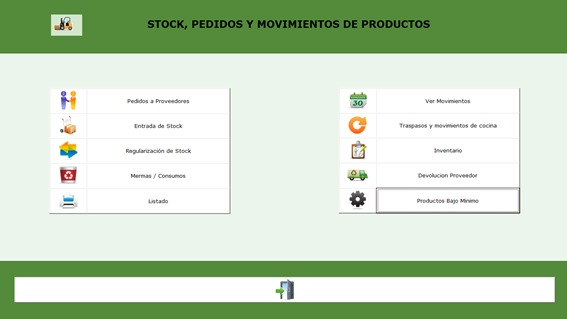
\includegraphics[scale=0.7]{8.jpg} 
 \end{center}
 \par\vspace{0.5cm}
\textbf {Configuración}\\\\
\begin{center}
 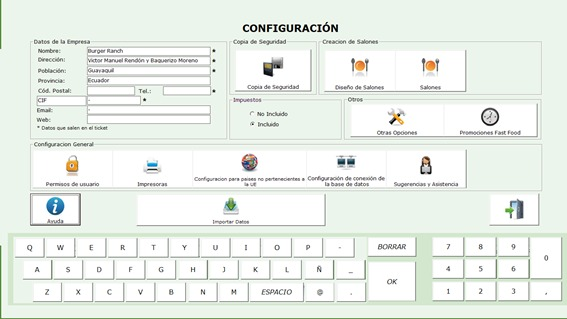
\includegraphics[scale=0.7]{9.jpg} 
 \end{center}
 \par\vspace{6cm}
\textbf {Listados}\\\\
\begin{center}
 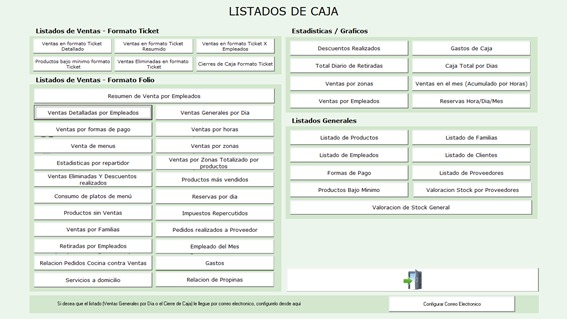
\includegraphics[scale=0.7]{10.jpg} 
 \end{center}
 \par\vspace{0.5cm}
 \textbf {Nivel de acceso}\\\\
\begin{center}
 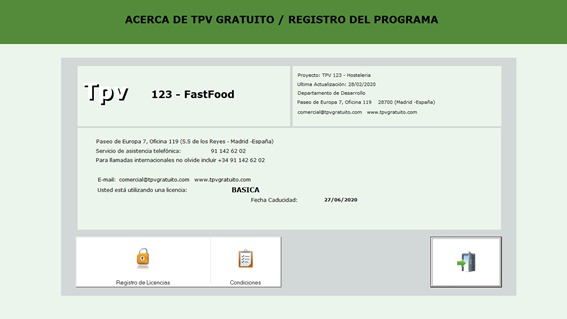
\includegraphics[scale=0.7]{11.jpg} 
 \end{center}

 \par\vspace{6cm}
\section{Evaluación del desempeño}\textbf{}
La empresa TPV 123 para evaluar el desempeño y eficacia del SGC tomó en cuenta las necesidades de los clientes, realizando seguimientos de las percepciones de los mismos para que de esta forma se cumplan las expectativas de los usuarios, estos seguimientos pudieron haber sido realizados mediante encuestas, retroalimentación del cliente sobre los productos y servicios entregados, reuniones con los clientes, análisis de las cuotas del mercado, informes comerciales, entre otros.\\

Los resultados de los análisis de la evaluación deben ver:
\begin{itemize}
\item {La conformidad de los productos y servicios.}
\item {El grado de satisfacción del cliente.}
\item {Si lo planificado se ha implementado de forma eficaz.}
\item {La eficacia de las acciones tomadas para abordar los riesgos y oportunidades.}
\item {El desempeño de los proveedores externos.}
\item {La necesidad de mejoras en el SGC.}
\end{itemize}
\section{Mejora}\textbf{}
El programa de TPV 123 FastFood cuenta con una versión actualizada, la cual contiene nuevas características como lo son:\\
\begin{itemize}
\item \textbf {Promociones 2x1, 3x2 y periodos de tiempo:} Ahora tienes la posibilidad de crear y aplicar ofertas, promociones, etc.
\item \textbf {Gestión de clientes:} Control al día de todo lo relacionado con tu cliente desde ventas, devoluciones, datos personales, envíos, llamadas, etc.
\item \textbf {Función multipuesto con varios equipos en tu red:} TPV 123 Fastfood te permite tener conectados en red varios puestos de trabajo en un mismo local.
De la misma manera continúa actualizando sus manuales de descarga y de uso, para brindar mayores facilidades a los usuarios que utilicen esta plataforma de venta.
\end{itemize}
\section{Referencia}\textbf{}
https://github.com/AlissonZambrano/ProyectoNormaISO.git
\end{document}
